\documentclass[authoryear,preprint,12pt,a4paper]{elsarticle}

\usepackage{amsmath,amssymb}
\usepackage{booktabs}
\usepackage{multirow}
\usepackage{tabularx}
\usepackage{graphicx}
\usepackage{xcolor}
\usepackage[colorlinks=true,linkcolor=blue,citecolor=blue,urlcolor=blue]{hyperref}

\journal{Computers in Industry}

\emergencystretch=1.5em
\tolerance=2000
\hyphenpenalty=50

\begin{document}

\begin{frontmatter}

\title{From agent goals to plant setpoints: configuration-driven governance
of LLM-agent writes on production lines}

% Double-blind submission: author metadata omitted.
\author[inst1]{Anonymous Author(s)}
\affiliation[inst1]{organization={Affiliation omitted for double-blind review}}

\begin{abstract}
Large language model (LLM) agent teams are beginning to operate on industrial
production lines, where they can read plant telemetry and issue supervisory
setpoint writes. Existing agent frameworks govern such actions at session
granularity. Such control cannot express plant semantics such as safe ranges,
recipe windows, or batch context, nor attribute a blocked or executed write
to a specific control. This paper treats the agent-to-plant write path itself
as the unit of governance. We present a configuration-driven platform in
which every machine-originated setpoint write must cross a sequence of
separately inspectable boundaries. These boundaries comprise a binding model
that scopes agent authority to plant nodes, and a four-layer admission
interval derived from node, parameter, product, and recipe configuration. A
human approval record binds the exact proposed operation and is rechecked at
dispatch time; a receipt grade distinguishes readback-verified from
transport-acknowledged writes. We evaluate the platform on five fronts. A
five-protocol device integration matrix on real protocol stacks passes 21/21
runner-defined checks. A four-arm ablation attributes interception of
window-breaching writes to the interlock layer, with zero false blocks on
the legitimate traffic. In a closed-loop case study, an LLM agent team
corrects melt pressure on a simulator-backed OPC UA line from 16.1 to
15.6\,MPa under human approval. In an adversarial episode, governance
cancels twelve out-of-surface model calls and journals them before any
unapproved write. The implementation is openly available, passes 913 of 915
unit tests, and reproduces its frozen ablation baseline bit-exactly across
twelve days.
\end{abstract}

\begin{keyword}
LLM agents \sep industrial cyber-physical systems \sep human-in-the-loop
control \sep production line governance \sep write access control \sep
OPC UA
\end{keyword}

\end{frontmatter}

\section{Introduction}
\label{sec:intro}

Production information systems are acquiring a new class of tenant. Industry
4.0 and Industry 5.0 framings place progressively more autonomy in the plant
while keeping human oversight central \cite{xu2021industry}. Beyond
the deterministic programs that have historically automated plants, large
language model (LLM) agent teams now read production telemetry, reason about
process state, and coordinate with each other over shop-floor tasks. These
agents inherit the reasoning and instruction-following capability of large
pretrained models \cite{zhao2023survey}. Recent
systems demonstrate LLM-based multi-agent orchestration on shop floors
\cite{zhao2026shopfloor}, LLM agents that operate industrial automation
systems \cite{xia2025control}, and LLM-driven control for skill-based
manufacturing \cite{koehle2026llmdriven}. Journal scopes that historically
hosted industrial informatics now explicitly name intelligent agents among
their enabling technologies. Application-oriented studies of LLM
assistants on assembly lines have appeared in this journal
\cite{llmdia2024}. The direction of travel is not in doubt: language-model
agents are moving from prototypes into the software stack that surrounds
production equipment.

Where these systems reach the equipment, they tend to encapsulate the action
inside a skill, a controller, or a validated proposal. The setpoint write
itself is different. A
supervisory setpoint write (changing a temperature setpoint, a pump speed,
a batch parameter) crosses from the information system into the physical
process. Its effect is delayed by process inertia, partially irreversible,
and intertwined with equipment-level protection that the information system
cannot see. Classical automation research has long warned about the
organizational, not merely technical, hazards of delegating control
\cite{bainbridge1983ironies}. Human-factors models place action
selection and execution at the stages where automation support changes
operator responsibility \cite{parasuraman2000model}. When the candidate
actor is an LLM agent, the delegation question becomes sharper: the agent is
capable, fallible, and susceptible to injected instructions
\cite{greshake2023injection,liu2024pinjection}.

Agent frameworks do govern actions, but at the wrong granularity for plants.
Session-level tool permissions decide \emph{whether} a tool may be called.
They do not encode \emph{plant semantics}: safe ranges, recipe windows,
batch context, and the one-proposal-per-actuator constraint are invisible
to them. Runtime
enforcement frameworks for LLM agents constrain tool calls by policies over
arguments \cite{wang2025agentspec}, and capability-based designs contain
prompt injection \cite{debenedetti2025camel}. Neither resolves which
control caught a given plant write. Neither binds a human approval to the
exact proposed operation under changing plant state, and neither
distinguishes a write that a device confirmed from one that a transport
layer merely acknowledged. On the industrial side, policy-governed agentic control
\cite{lin2026agentic} and P\&ID-grounded validation \cite{schall2026safe}
show that governance is recognized as necessary. Yet the audit question
remains open: when a write is blocked or executed, an engineer must be able
to see \emph{which layer} decided, on \emph{which configuration}, with
\emph{what receipt}.

A running example makes the unit of governance concrete. An agent observes
a melt-pressure excursion and proposes $130\to127$\,rpm. The value is
inside the node's hard engineering range, but the active recipe window and
the one-proposal-in-flight rule must also be consulted, and a second team
may already hold an opposing proposal. The platform binds the request to
the current line--product--recipe--run tuple, returns a typed verdict that
names any excluding layer, asks a human to approve the exact value and
applicable limits when the binding is manual, rechecks the tuple at
dispatch, reads the value back, and records the receipt grade and every
decision in the ledger. This is the path that Sections~\ref{sec:arch}
and~\ref{sec:eval} evaluate; the rest of the paper explains why each
boundary is necessary and what evidence supports it.

This paper takes the agent-to-plant write path itself as the unit of
governance. We present a configuration-driven platform in which LLM agent
teams and a production line share one runtime, and in which every
machine-originated setpoint write must cross a sequence of separately
inspectable boundaries. A binding model scopes agent authority to plant
nodes. A four-layer admission interval is formed by intersecting the node's
hard engineering range with parameter, product, and recipe limits. A human
approval record is bound to the exact proposed values, applicable limits,
and the active line--product--recipe--run tuple, and is rechecked at
dispatch time. A receipt grade separates readback-verified writes from
transport-acknowledged and unverified ones. Every decision on this path,
including every rejection, is recorded in an auditable ledger. The design
intentionally makes attribution and prevention separable: a layer that
cannot block still records, and a layer that blocks states why.

We evaluate the platform across five question areas, each backed by
re-runnable evidence artifacts. A five-protocol device integration matrix
(Modbus TCP, Modbus RTU, OPC UA, MQTT, HTTP) on real protocol stacks passes
21 of 21 checks, including platform-versus-device readback equality and
honest failure on disconnects. A four-arm ablation isolates which layer
provides interception of window-breaching writes: removing the soft
batch-window interlock lets six attack writes execute (all journaled), while
the hard engineering range produces zero false blocks in every arm. A
closed-loop case study on a simulator-backed OPC UA line (real protocol
stacks, simulated process physics) shows an LLM agent team (running a
9B-class open model through a standard harness) moving melt pressure
from 16.1 to 15.6\,MPa with two human approvals, an
agent-self-calibrated process gain, and an independent physical recheck. An
adversarial episode with the same weak model class ends with the platform
canceling the task after recording twelve tool-surface violations and nine
unapproved harness calls, with zero unapproved writes. Finally, the open
implementation passes 913 of 915 unit tests and reproduces a frozen
benchmark baseline bit-exactly across twelve days.

The contributions are:
\begin{enumerate}
\item \textbf{Configuration-driven binding model.} A configuration model
that binds agent authority to production context (lines, products,
recipes, runs, and nodes) and injects derived semantic context into agent
prompts, so that write scope is a configuration fact rather than a prompt
convention (Section~\ref{sec:arch-binding}).
\item \textbf{Layer-attributable governed write path.} A write path that
admits setpoint writes through a four-layer interval, bound human approval
with tuple recheck, and receipt-graded verification, and that records every
admission decision (execution or rejection) with the deciding layer
identified (Section~\ref{sec:arch-write}).
\item \textbf{Multi-level evaluation with mechanism attribution.} An
evaluation combining device-level protocol integration, a four-arm ablation
that attributes interception to a specific layer with zero false blocks, a
real LLM-agent closed-loop case study, a model-driven optimization tier, and
an adversarial episode (Section~\ref{sec:eval}).
\item \textbf{Deployable open implementation.} A single-runtime
implementation distributed as an installable package, with five industrial
connectivity protocols, fourteen agent harness adapters, 913 of 915 unit
tests passing, and bit-exact frozen-baseline reproduction
(Section~\ref{sec:impl}, Section~\ref{sec:eval-quality}).
\end{enumerate}

The remainder of this paper is organized as follows.
Section~\ref{sec:related} reviews LLM agents in industrial systems and
governance for machine-originated actions. Section~\ref{sec:problem} states
the failure model and requirements. Section~\ref{sec:arch} presents the
architecture and the governed write path. Section~\ref{sec:impl} describes
the implementation and deployment. Section~\ref{sec:eval} reports the
evaluation. Section~\ref{sec:discussion} discusses implications, limitations,
and threats to validity, and Section~\ref{sec:conclusion} concludes.

\section{Related work}
\label{sec:related}

\subsection{LLM agents in industrial systems}
\label{sec:related-agents}

A growing body of work connects LLM agents to production equipment. At the
execution level, an agent turn interleaves reasoning with tool invocation
\cite{yao2023react}, and models can be taught to call tools
\cite{schick2023toolformer}; the governing question is therefore not
whether an agent can invoke an operation but what bounds that invocation.
Architectural studies integrate LLMs with digital twins and automation
systems \cite{xia2025architecture} and with asset administration shells and
OPC UA information models \cite{graul2026aas}. Control-facing systems use
LLM agents to operate automation systems \cite{xia2025control}, to explore
resource capabilities in multi-agent manufacturing
\cite{lim2025llmenabled}, to drive skill-based manufacturing control
\cite{koehle2026llmdriven}, and to compose semantic recipes on OPC UA
skills \cite{koehle2025semanticrecipes}. Shop-floor orchestration systems
coordinate multi-agent LLM teams for manufacturing tasks
\cite{zhao2026shopfloor}, and pretrained LLMs have been placed in the loop
of robot-operated serial production lines \cite{waseem2026pretrained}.
Process-industry studies use LLM agents with digital twins for fault
handling \cite{gill2025llmdt} and natural-language machine operation over
OPC UA \cite{hofmann2025nlc}. Reviews of agentic AI for process monitoring
and fault diagnosis \cite{jiang2026agentic} and of LLM-enabled digital
twins \cite{gill2025llmdt} catalog the application space. Closer to control
theory, InstructMPC embeds human--LLM interaction into context-aware MPC
\cite{wu2025instructmpc}, and LLM-based architectures have been proposed
for automated control-code generation in industrial cyber-physical systems
\cite{huang2026made} and closed-loop PLC code generation with verification
\cite{liu2026agents4plc}. This journal has hosted platform papers of
comparable shape, including an open-source compositional digital twin
framework \cite{opentwins2023} and requirements and design patterns for
adaptive digital twins \cite{dtpatterns2023}, as well as a controlled
assessment of an LLM-based digital intelligent assistant in assembly
manufacturing \cite{llmdia2024}.

Across these systems the LLM occupies one of two positions. In
\emph{advisory} positions the agent reads state and recommends; a human or a
conventional controller acts. In \emph{actuating} positions the agent's
output reaches equipment directly \cite{waseem2026pretrained,
xia2025control,koehle2026llmdriven,hofmann2025nlc}. The actuating position is
where governance matters most, and it is the position this paper addresses.

\subsection{Governing machine-originated actions}
\label{sec:related-gov}

Human-factors research frames the delegation of action to automation as a
allocation problem across types and levels of human interaction
\cite{parasuraman2000model}, and warns that human oversight of a
predominantly automatic system degrades through complacency and bias
\cite{parasuramanmanzey2010complacency,bainbridge1983ironies}. These
results motivate designs in which the human decision is exercised against a
concrete, inspectable proposal rather than a summary. In the agent-safety
literature, runtime enforcement systems constrain LLM agent behavior with
user-defined rules \cite{wang2025agentspec}; capability-based architectures
defeat prompt injection by construction \cite{debenedetti2025camel};
benchmarks formalize injection attacks and defenses
\cite{liu2024pinjection,zhan2024injecagent} and dynamic environments
evaluate attacks and defenses against tool-using agents
\cite{debenedetti2024agentdojo}, demonstrating that agents that read
plant-facing content are exposed to manipulated instructions. Industrial
security standards contribute the zone-and-conduit model
\cite{iec62443-3-2} and system security requirements
\cite{iec62443-3-3}, and safety instrumented systems define the
plant-side final barrier \cite{iec61511}; both assume the information
system's requests arrive through designed channels, which is exactly the
assumption an unconstrained agent violates. Architectural work on
digital-twin-based automation security \cite{gehrmann2020dtiacs}, secure
fog layers for the industrial IoT \cite{sengupta2021securefog}, and
functional architectures for special-purpose industrial networks
\cite{mahmood2023functional} shows that separating concerns across layers
is an established design idiom for industrial trust boundaries.

On the industrial side, Lin et al.~\cite{lin2026agentic} integrate policy-governed
agentic AI with multi-source sensor--MES--ERP data for closed-loop
manufacturing control, and Schall~\cite{schall2026safe} validate LLM proposals
against P\&ID-derived structure before they reach process control.
Biskupovic et al.~\cite{biskupovic2025supervision} realize agent-based supervision for
service-oriented industrial cyber-physical systems. These works establish
that plant writes need governance. What remains under-specified is the
audit dimension: the ability to answer, after the fact, \emph{which layer}
of the path admitted or rejected a specific write, against \emph{which
configuration revision}, and with \emph{what device-side receipt}. Existing
descriptions typically report governance as a property of the overall
pipeline; they do not separate the layers, nor grade the evidence that a
write actually took effect.

Two honest boundaries on this positioning should be stated. First,
\emph{the individual mechanisms have industrial precedents}: limit
checking against engineered ranges, post-write verification, and
approval workflows with audit trails are established practice in
process control and regulated industries (cf. electronic-record audit
trail requirements such as 21 CFR Part 11), and run-to-run control
already bounded recipe execution decades ago \cite{moyne2000r2r}. The
contribution claimed here is not any single mechanism but their
configuration-driven composition into one agent-facing path in which
every layer's verdict is separately recorded, the deciding layer of a
rejection is identifiable, receipts are graded by device-side evidence,
and no bypass exists from the agent surface. Second, \emph{a conservative
alternative exists}: keeping the LLM strictly read-only and leaving
writes to conventional DCS limits plus historian audit covers much of
the same ground when actuating agents are not wanted. The platform's
value proposition is for deployments that \emph{do} want supervised
agent-initiated writes, where it makes such writes governed by
construction rather than by convention. Table~\ref{tab:position}
positions representative systems along this dimension.

\begin{table}[!t]
\centering
\caption{Representative LLM-agent industrial systems and their treatment of
plant-facing writes (characterizations at citation level, from the cited
works' stated scope).}
\label{tab:position}
\small
\begin{spacing}{1.0}
\begin{tabularx}{\columnwidth}{@{}p{0.24\columnwidth}p{0.30\columnwidth}X@{}}
\toprule
Study & LLM role & Plant-facing write treatment \\
\midrule
Zhao et al.~\cite{zhao2026shopfloor} & Shop-floor multi-agent orchestration & Task-level coordination; not centered on setpoint writes \\
Xia et al.~\cite{xia2025control} & Operates automation systems & Direct system operation; engineering limits not the focus \\
K{\"o}hle et al.~\cite{koehle2026llmdriven} & Skill-based control & Skill invocation; skills encapsulate equipment access \\
Lin et al.~\cite{lin2026agentic} & Policy-governed closed-loop control & Policies govern agent actions in the control loop \\
Schall~\cite{schall2026safe} & Process-control integration & P\&ID-grounded validation of proposals \\
Wu et al.~\cite{wu2025instructmpc} & Context provider for MPC & Human--LLM interaction around a conventional controller \\
Hofmann et al.~\cite{hofmann2025nlc} & Natural-language operation & NL commands mapped to OPC UA operations \\
\midrule
This work & Supervisory agent teams & Layer-attributable interlocks, bound approvals, receipt grading, audited ledger \\
\bottomrule
\end{tabularx}
\end{spacing}
\end{table}

\section{Problem statement and requirements}
\label{sec:problem}

We consider a production line supervised by an information platform that
provides data acquisition from plant nodes and controlled writes to plant
nodes, in the sense of the enterprise--control integration models of
ISA-95 \cite{isa95_2025} and batch control models of ISA-88
\cite{isa88_2010}; the line--product--recipe--run tuples used throughout
this paper correspond to ISA-88 control-recipe and batch identities. LLM
agent teams run inside the same platform. Each team
is led by a coordinator agent that decomposes a stated production goal into
worker tasks; agents perceive the plant through queries against acquired
telemetry and act through platform operations. We do not consider
real-time control loops: the platform occupies a supervisory position in
which decisions occur on second-to-minute cadences, and equipment-level
protection remains with the plant's own basic process control and safety
instrumented systems \cite{iec61511}. The platform is not a safety
barrier and makes no claim inside a safety-instrumented function.

\subsection{Failure model}
\label{sec:problem-fm}

Four failure classes motivate the design. They are stated from the plant
operator's perspective: each is an event that can occur, that operators must
afterwards reconstruct, and that current agent frameworks make difficult to
reconstruct.

\textbf{M1: Unconstrained machine-originated write.} An agent issues a
setpoint write that violates plant engineering context: outside the
node's safe range, outside the recipe window of the product currently in
production, or in conflict with another proposal in flight. Session-level
tool permissions cannot see this context: the write tool is either allowed
(and the violation passes) or denied (and no legitimate write is possible).

\textbf{M2: Unattributable decision.} A write is blocked (or executes)
and the operator cannot determine which control decided. If scope checks,
engineering interlocks, and approval requirements are evaluated in one
amalgamated policy, the audit log records an outcome but not its cause.
Attribution matters operationally: a block caused by an expired approval
window is fixed differently from one caused by a recipe window.

\textbf{M3: Stale or replayed approval.} A human approves a proposed write;
plant state changes before the write executes (a different recipe starts, a
batch closes, limits are revised); the write executes under the old
approval. The approval was real, but it no longer describes the operation
performed.

\textbf{M4: Unverified receipt.} The platform reports success because a
protocol stack acknowledged a transmission. The device may not have applied
the value. A readback would have shown so. Operators who rely on the
transport acknowledgment form beliefs about plant state that the device does
not support.

Prompt injection sharpens all four classes: an agent that reads plant-facing
content can be steered to request writes it was never asked for
\cite{greshake2023injection,liu2024pinjection}. The path must therefore
treat the \emph{requester} as untrusted even when the request is
well-formed.

\subsection{Requirements}
\label{sec:problem-req}

From the failure model we derive six requirements for a governed write path.

\textbf{R1 (Context-encoded scope).} Agent authority over writes must be a
configuration fact (bound to specific nodes, expressible per point, per
recipe, or per line) and must derive from plant structure (lines,
products, recipes, runs), not from prompt conventions.

\textbf{R2 (Layered admission).} Every write must cross an admission
interval formed by independent layers: a structural hard range at the node,
then parameter, product, and recipe limits. Layers must be evaluated in a
fixed order and the first excluding layer must be identifiable.

\textbf{R3 (Defense in depth).} No single layer may be load-bearing for
safety. If one layer is disabled or misconfigured, remaining layers must
still bound writes, and the hard node range must be bypassable by no
configuration flag.

\textbf{R4 (Bound, rechecked approval).} When a binding requires human
approval, the approval must record the proposed values, the applicable
limits, an expiry, and the active line--product--recipe--run tuple; the
dispatching stage must recheck the record against current state before
executing, so that M3 fails closed.

\textbf{R5 (Honest receipts).} Write outcomes must be graded into at least
three classes (readback-verified, transport-acknowledged, and unverified),
and the platform must not represent a transport acknowledgment as
device-side confirmation.

\textbf{R6 (Total audit).} Every admission decision, including every
rejection with its deciding layer, must be recorded in an append-only
ledger, so that M2 fails closed: an absent record is itself evidence.

R1--R2 address M1; R2's layer ordering plus R6 address M2; R4 addresses M3;
R5 addresses M4; R3 constrains the whole chain. Section~\ref{sec:arch}
presents the architecture that realizes these requirements, and
Section~\ref{sec:eval} evaluates them, including a four-arm ablation
designed to attribute interception to specific layers (R2--R3) and to
measure false blocks, the cost side of governance.

\section{System architecture}
\label{sec:arch}

\subsection{Runtime overview}
\label{sec:arch-overview}

Figure~\ref{fig:arch} shows the platform. Three cooperating sides share one
runtime process. The \emph{agent collaboration runtime} hosts workspaces,
channels, agent teams (a lead that decomposes goals and supervises workers,
plus workers that execute tasks), per-channel event buses with sequenced
delivery, shared process memory, and mailboxes. Agents are executed by
pluggable \emph{harness adapters}. Fourteen adapters cover in-process
engines, RPC subprocess engines, ACP-style engines, served engines, and
headless CLI engines, so that the same governed operation surface is
exposed regardless of which LLM backend a team runs. The \emph{governance
block} holds the operation catalog and the per-call checks described in
this section. The \emph{industrial side} comprises the data-acquisition
gateway with per-node edge runtimes, the write-control gateway, protocol
drivers for five field protocols plus a serial plugin and a MES REST
integration, and the time-series store. The store is embedded SQLite by
default, or TimescaleDB with daily chunks and compressed columnstore when
provisioned.

\begin{figure}[!t]
\centering
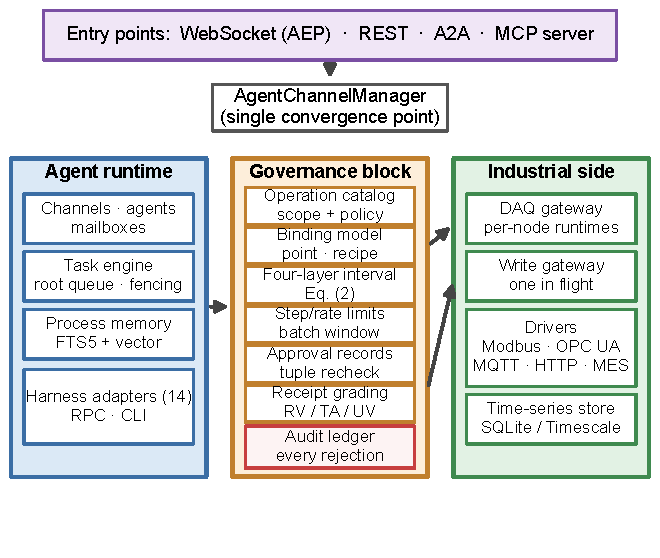
\includegraphics[width=0.98\columnwidth]{figures/fig1-architecture.pdf}
\caption{Platform architecture. Agent teams run inside the collaboration
runtime through pluggable harness adapters; all plant-facing operations
cross the governance block, which evaluates binding scope, the four-layer
admission interval, approval records, and receipt grading, and writes every
decision to the audit ledger. The industrial side separates acquisition
from write control and persists telemetry in an embedded or provisioned
time-series store.}
\label{fig:arch}
\end{figure}

Four entry points (WebSocket, REST, A2A, and an in-process MCP server
\cite{mcp2024,silva2025mcpmanufacturing}) converge on the same
AgentChannelManager, so that an operation is governed identically no matter
where it originates. This convergence is deliberate: it prevents the
common failure mode in which an interactive path is governed but a
programmatic path is not.

\subsection{Configuration-driven binding model}
\label{sec:arch-binding}

\textbf{Production context as configuration.} The platform's configuration
model describes the plant as \emph{scenes}: a scene declares lines; a line
declares products; a product declares recipes; a recipe declares
parameters with engineering windows. A line run instantiates a
line--product--recipe tuple and opens a batch. Nodes are typed as
acquisition nodes (readable plant points) or write-control nodes
(writable plant points). Each carries protocol driver configuration, a
structural safe range, and semantic metadata (meaning, unit, engineering
interpretation). All of this is data (one declarative source with
declared defaults), not code. A running configuration therefore answers,
for any moment, \emph{what is being produced, under which recipe, with
which windows, on which nodes}.

\textbf{Agent authority.} Agent authority is bound to this structure
through three binding tracks. A \emph{point binding} ties an agent to
specific write-control nodes; the set of values an agent may dispatch is
the intersection of the requested set with the bound set, so a binding
narrows rather than grants. A \emph{recipe binding} grants operations on a
single recipe; a \emph{line-recipe binding} grants operations across all
recipes of a line. Binding modes are \emph{manual} (every dispatch waits
for human approval) or \emph{auto}; switching a binding to auto requires an
explicit confirmation action, never a side effect of normal use.
Separately, users hold tri-state line permissions (none, view, operate);
the data plane filters by permission before any agent-level check, so an
agent bound to a node the user cannot operate still yields no data.

Direct node-write operations are refused by design: the tool family that
would bypass the governed path exists only as a single-source declaration
whose handlers reject unconditionally, keeping the write path non-bypassable
from the agent surface. Agent-facing tool descriptions are injected from
the same configuration (semantic cards derived from node metadata, line
condition, and associated devices). Thus, the agent's view of a node
carries its engineering meaning, and the model is not trusted to have
remembered it.

\textbf{Shared dispatch condition.} Every plant-facing operation request
$(a, c, u)$ (agent $a$, capability $c$, and unit of work $u$) is
admitted by a conjunction of predicates drawn from the governance block:
\begin{equation}
\mathcal{A}(a,c,u) \;=\; \bigwedge_{X \in \mathcal{C}(u)} X(a,c,u),
\qquad \mathcal{C}(u) \subseteq \{S, P, G, B\},
\label{eq:dispatch}
\end{equation}
where $S$ is scope (the agent holds the binding for $c$ on $u$), $P$ is the
channel policy under which $a$ runs, $G$ is any applicable grant, and $B$
is the operation-specific binding predicate. $\mathcal{C}(u)$ always
contains $S$ and $P$; $G$ and $B$ attach for the write-path operations
discussed next. Each predicate records its own verdict, which is what makes
the eventual audit layer-attributable rather than binary.

\subsection{The governed write path}
\label{sec:arch-write}

Figure~\ref{fig:writepath} traces a setpoint write through the path. The
stages realize R2--R6. Individually, these mechanisms have precedents in
industrial practice: engineered-range limit checks, post-write
verification, approval workflows with audit trails. What follows states
them precisely so that their \emph{composition} can be evaluated rather
than assumed: the composition adds separately attributable verdicts,
receipts graded by device-side evidence, and the absence of a bypass from
the agent surface.

\textbf{Walkthrough.} The running example of Section~\ref{sec:intro} is
admitted in five observable steps. (i)~R1: the binding query resolves the
node and the recipe; a missing binding rejects before any driver call.
(ii)~R2--R3: the four-layer interval intersects the node's hard range with
the active product and recipe windows; a value outside the intersection
returns the excluding layer, and the hard range is never administratively
relaxed. (iii)~R4: a manual binding creates an approval record carrying the
candidate value, the applicable limits, an expiry, and the
line--product--recipe--run tuple; dispatch rechecks the tuple and limits.
(iv)~R5: the driver executes; the platform reads the value back and grades
the receipt, reporting a transport acknowledgment as such. (v)~R6: every
prior verdict, including the rejection path, is appended to the ledger.
The example is deliberately ordinary: the design claim is that no step can
be skipped from the agent surface.

\begin{figure}[!t]
\centering
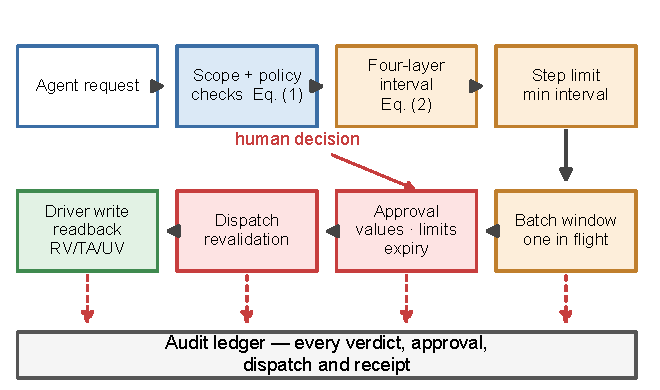
\includegraphics[width=0.98\columnwidth]{figures/fig2-writepath.pdf}
\caption{The governed write path. A machine-originated setpoint write
crosses scope and policy checks, the four-layer admission interval, rate
and step limits, a human approval record with tuple recheck, dispatch-time
revalidation, driver execution, readback verification, and receipt grading;
every stage's verdict, including rejections, lands in the audit
ledger. Rejection paths are drawn dashed.}
\label{fig:writepath}
\end{figure}

\textbf{Four-layer admission interval.} For a write-control node $n$ at
time $t$, the admissible value interval is
\begin{equation}
\mathcal{I}^{\mathrm{online}}_n(t) \;=\;
\mathcal{H}_n \;\cap\; \mathcal{L}^{\mathrm{base}}_n
\;\cap\; \mathcal{L}^{\mathrm{prod}}_n(t)
\;\cap\; \mathcal{L}^{\mathrm{rec}}_n(t),
\label{eq:interval}
\end{equation}
the intersection of the node's hard engineering range $\mathcal{H}_n$
(structural, not administratively relaxable), the parameter baseline
limits, the limits of the product currently in production, and the
parameter window of the recipe currently in production. A value outside
the intersection is rejected, and the response identifies the excluding
layer. The layers are evaluated in this fixed order, so two writes
rejected by different layers produce observably different records (M2).

\textbf{Rate and step limits.} Online writes additionally pass a per-node
step limit (a node without a configured step limit rejects online writes
rather than inheriting a default), a minimum interval between successive
writes, and a cooldown after a failed write. These limits apply
uniformly across protocol drivers; a driver cannot opt out.

\textbf{Batch-window interlock.} When a line run is active, writes are
admitted only within the run's batch window, and only one proposal per
actuator may be in flight. A second proposal, even from a different
agent team, waits or is refused, and a human arbitrates conflicting
intents. This interlock is deliberately \emph{soft}: it is the layer the
evaluation ablates (Section~\ref{sec:eval-ablation}), which requires that
the platform can run with it disabled. Disabling it does not disable the
hard range: R3 is preserved by construction, and the ablation confirms it
empirically.

\textbf{Bound approval.} For bindings in manual mode, the write dispatch
suspends and an approval record is created. The record binds the requesting
actor, the proposed operation and candidate values, the applicable limits
at proposal time, an expiry (a configurable setting; default 180\,s, with
the decision defaulting to rejection on timeout), and the active
line--product--recipe--run tuple. The
human approves or rejects in a dedicated surface; the platform never
writes on the agent's behalf while approval is pending. Recipe-level
operations (promoting a full parameter set) carry a separate, stricter
approval gate with the approver's stated basis returned verbatim into the
record.

\textbf{Dispatch-time revalidation.} Approval is not a capability token.
At dispatch, the path revalidates the approver's authority and compares
the current line--product--recipe--run tuple, the applicable limits, and
the approval expiry against the record; any mismatch fails the dispatch
closed (M3). The same revalidation runs again at the execution point after
queueing, bounding the window between decision and device contact.

\textbf{Receipt grading.} After driver execution the platform grades the
outcome. Where the driver provides a read channel, the written value is
read back (a mismatch triggers up to three re-reads at 2\,s intervals to
absorb actuator settling). The receipt is then \emph{readback-verified}.
A protocol-level success status alone does not qualify: an OPC UA Write
service result, for instance, reports server-side application rather than
physical effect, which is precisely why the top grade requires a readback.
Where the integration path provides only an acknowledgment, the receipt is
\emph{transport-acknowledged}; the platform states explicitly that this
class does not establish that the device applied the value. Where neither
exists, the receipt is \emph{unverified}. Downstream consumers, including
agents, receive the grade with the result text, so a report that cites a
write also cites its evidence class (M4).

\textbf{Total ledger.} Every stage verdict is appended to the audit ledger:
admission decisions with the deciding layer and excluding interval, approval
creations, approvals and rejections with actor and basis, revalidation
failures, dispatch attempts, and receipts with grades. Rejections are
first-class records, not silent drops. The ledger is the substrate for
Section~\ref{sec:eval-ablation}'s mechanism attribution: an ablation arm
can be shown to have executed window-breaching writes \emph{because the
ledger says so}, even when the platform had no power to stop them.

\subsection{Acquisition, context, and agent runtime}
\label{sec:arch-daq}

On the read side, each acquisition node runs an edge runtime with an
ingest cadence and an independent publication cadence (capped for
interface backpressure). A gateway sweeps drivers on a fixed 250\,ms
cycle with in-flight mutual exclusion, drops out-of-order frames, and
rejects future timestamps rather than persisting them. Persistence is
gated on an \emph{active batch}: telemetry outside an active line run is
served live but not written to history, which keeps the analytical store
aligned with production context. Recipe-window breaches observed on
acquired values raise alarm edges from the same runtime that persists
samples, so monitoring and history cannot diverge.

Agents perceive the plant through a bounded tool surface: history queries
with statistics, current-value reads, node discovery scoped by bindings,
and the governed write operations of
Section~\ref{sec:arch-write}. The task runtime is a seven-state machine
(SUBMITTED, ASSIGNED, WORKING, WAITING, COMPLETED, FAILED, CANCELED) with a
root-queue and lease fencing; leads re-dispatch failed tasks under budget.
A regulation workflow template (observe, understand, hypothesize,
propose, await decision, verify, review) is injected into supervisory
prompts together with the semantic cards of Section~\ref{sec:arch-binding}.
Its constraint set (goals must land inside the safe range intersected
with the recipe window; single steps bounded to a small fraction of the
range) mirrors the path's own limits. The agent is thus asked to do
nothing the path would refuse.

\subsection{Model-driven optimization tier}
\label{sec:arch-opt}

Agents do not have to propose setpoints from raw reasoning alone. An
optional model tier (automated machine learning over acquired process
data) produces process models that agents can solve against. The tier is
gated so that model quality claims are platform-recomputed rather than
self-reported. Training jobs produce candidates. Promotion to
reference-grade status requires passing a gate set that includes
single-step and rolling prediction error bounds, a generalization gap
bound, and minimum data-volume requirements, evaluated by the platform on
held-out data. Uncertainty calibration (conformal bounds over a residual
ensemble on top of a physics-prior core with clamped residual scale) and
out-of-distribution rejection are part of the model contract. A trial
service simulates candidate setpoint moves against a gated model before
any plant contact and marks trial outcomes as simulation evidence;
candidates that pass a twin gate may then be bound to a channel, and only
bound models enter the optimizer surface.

The optimizer itself compiles a problem intermediate representation with a
content hash (model artifacts, MV domains taken strictly from node specs
including step limits, CV targets) and solves it with OSQP over a dense
sensitivity expansion, with movement and hard-domain constraints. A
steady-state variant uses SLSQP. Two independent services, the solver
and the digital twin \cite{jones2020characterising}, recompute the same
objective from the same frozen
inputs and must agree to within $10^{-6}$ relative tolerance before a
result is surfaced; model artifact hashes are cross-checked, so the
dual-check cannot silently span different model revisions. Dispatched
recommendations re-enter the governed write path of
Section~\ref{sec:arch-write}: the optimizer has no private path to the
plant. Recipe trials run at a bounded cadence with a declared hypothesis;
an outcome that meets the hypothesis promotes the recipe version (with a
second human approval). One that does not rolls back through a
unified rollback service that restores the previous version and, where the
driver supports it, rewrites the affected plant values as a batch. Judge
and executor are separate services, so the component that decides a trial
failure is not the component that performs the rollback.

\section{Implementation and deployment}
\label{sec:impl}

The platform is implemented as a single server runtime in TypeScript on
Node.js, with a Vue 3 front end. One process hosts the four entry points
(HTTP, WebSocket, A2A, MCP), the agent runtime, and the industrial stack;
there is no separate governance service to deploy or bypass. State lives
in an embedded SQLite database (via the Node built-in driver) by default;
when production-grade history is required, a provisioned deployment adds a
TimescaleDB (compressed, chunked daily) and an MQTT broker, and the
acquisition gateway switches its storage backend without changes to the
governed path.

\textbf{Protocol surface.} Five industrial connectivity protocol drivers
are built in:
Modbus TCP, Modbus RTU, OPC UA \cite{iec62541}, MQTT, and HTTP, plus a
serial-port plugin driver and a MES REST integration with mirror and live
modes. Drivers implement a common read/write contract, so admission
limits, approval, and receipt grading apply uniformly; a driver cannot
weaken them. Write nodes carry per-driver configuration (register maps,
byte order, scaling, topic maps) declared once in the scene configuration.

\textbf{Agent harness surface.} Fourteen harness adapters execute agent
teams: two in-process engines (a deterministic mock for testing and a
Claude-compatible engine), an RPC-subprocess engine, an app-server engine,
three ACP-style engines, a served engine, and six headless CLI adapters.
The registry normalizes turn execution and tool invocation, so the
governed operation surface is identical across engines; an episode can mix
engines per channel. Teams are described declaratively (lead and worker
roles, model preferences) and instantiated from templates.

\textbf{Configuration and extension.} A single configuration schema feeds
defaults (a YAML file), runtime overrides, and environment variables;
settings and their descriptions are declared once and consumed by both the
settings UI and the CLI. A hot-reloadable plugin surface registers
additional drivers, processors, node templates, agent tools, HTTP routes,
browser panels, twin providers, and line-permission hooks; a failing
plugin is isolated from the runtime. The platform ships as an installable
npm package with an \texttt{aw} CLI (\texttt{aw start} initializes a home
directory, migrates prior versions, and serves the UI); production
posture terminates TLS on a reverse proxy in front of the single service.
The host tool surface exposed to agents comprises 105 built-in tools plus 21
plugin-registered tools (126 at the evaluated release), including the
industrial operations used in this paper; every tool's description and
scope semantics are generated from the same operation catalog that the
governance block enforces.

\textbf{Evidence pipeline.} All experiments in Section~\ref{sec:eval} are
driven by a benchmark pipeline in the same repository. A runner provisions
scenes through the platform's own REST surface, executes scenario scripts,
and freezes a report, raw event logs, and checksums into a versioned
results directory. Each result records the runner command, source commit,
and harness hash, which is what enables the frozen-baseline reproduction
checks of Section~\ref{sec:eval-quality}.

\textbf{Deployment posture and its boundaries.} The single-process design
places the agent runtimes (including outbound-capable harness adapters) and
the protocol write drivers in one trust domain. That is a deliberate
simplicity for evaluation, but it does not by itself satisfy IEC 62443-3-2
zoning. A plant deployment should place the platform inside a defined zone
with conduits to the control network, isolate harness adapters from
field-facing interfaces, and provide backup and restart procedures. Node
version, resource sizing, and high-availability specifications are
deployment-engineering tasks this paper does not claim; harness-side
isolation, air-gapped packaging, and a zoned reference architecture are
future work (Section~\ref{sec:conclusion}).

\section{Experimental evaluation}
\label{sec:eval}

\subsection{Method and evidence discipline}
\label{sec:eval-method}

We structure the evaluation around five research questions:

\begin{itemize}
\item \textbf{RQ1 (Integration).} Can one configuration-driven runtime
integrate heterogeneous plant protocols such that platform-side data and
write paths equal device-side behavior, including under faults?
\item \textbf{RQ2 (Mechanism attribution).} Which layer of the write path
provides interception of policy-breaching writes, does removing a layer
degrade safety, and does governance introduce false blocks?
\item \textbf{RQ3 (Closed loop).} Can an agent team complete a governed
supervisory correction (read, analyze, propose, human approval, write,
readback, retest, record) end to end on a running line?
\item \textbf{RQ4 (Model-driven tier).} Does the model-driven optimization
tier respect the same governance and improve closed-loop performance in
simulation?
\item \textbf{RQ5 (Adversarial containment).} How does the platform behave
when a real, weak open-weight model attempts out-of-surface actions?
\end{itemize}

Every experiment is executed by a benchmark runner in the platform
repository and freezes a report, raw event logs, and SHA-256 checksums
into a versioned results directory that records the runner command, source
commit, and harness hash. Two plant scenarios are used: a cast-film line
driven by a physical-engine simulator (first-principles actuator and
material dynamics) with a MES mirror, and an injection line driven by a
PLC node simulator exposing all five protocols. LLM episodes use the omp
RPC harness serving an open-weight 9B-class model (Qwen3.5-9B, 64k
context, locally served); integration and ablation runs are deterministic
(no LLM) by design, so that mechanism-level results are not confounded by
model stochasticity. We report negative and mixed outcomes alongside
positive ones; none of the results below pool runs across scenarios into
a single denominator.

\subsection{Device integration across five protocols (RQ1)}
\label{sec:eval-integration}

The device integration matrix connects real protocol stacks (Modbus
TCP, Modbus RTU, OPC UA, MQTT, and HTTP) to the virtual PLC and
exercises the full path from configuration to write. The matrix passes
21 of 21 assertions (Table~\ref{tab:integration}): environment
self-checks, scene provisioning, per-protocol acquisition with
platform-versus-device value equality, write-through on the four writable
protocols with dispatch narrowing, negative probes, and fault handling.
In fault handling, a disconnect is reported honestly as a failure and the
path self-heals on reconnect. A companion provisioning run on a second scene
(an injection line with thirteen acquisition nodes including a vector
profile node, plus three write nodes) brought all thirteen acquisition
nodes online through the same configuration surface with no code change.

A longer integrated pipeline run (one deterministic execution covering
scene provisioning, acquisition, governed operations, seeded objective
cases, a second scene, and a scripted BOPET task) passed all 17 phase
gates and 76 of 77 checks (one warning on a semantic-card check; zero
failures). Within that run, five protocol endpoints returned 54 samples,
and all 24 negative probes on four writable paths were rejected before
driver execution. A second-scene configuration rejected 9 of 9 additional
probes. The median write round-trip across the four writable protocols
was 31.6\,ms including real protocol transactions. Three
fixed-seed objective cases solved against the simulator's offline
reference ended at 96.3--98.8\% of the reference (mean 97.8\%); one seed
began inside the stopping region and correctly terminated with zero
writes. This run demonstrates configuration breadth and regression
fidelity; the matrix above demonstrates real-stack fidelity.

\begin{table}[!t]
\centering
\caption{Device integration matrix on real protocol stacks (21/21
assertions pass). Grouped view of the frozen assertion set; every group
passed in full.}
\label{tab:integration}
\small
\begin{spacing}{1.0}
\begin{tabularx}{\columnwidth}{@{}p{0.34\columnwidth}X@{}}
\toprule
Group & What is checked \\
\midrule
Environment (S0--S1) & Simulator and platform reachable; scenario baseline valid \\
Provisioning (P0--P2) & Scene configuration provisions lines, products, recipes, nodes through the platform API \\
Acquisition (D--*, D-match) & Per-protocol sampling on Modbus TCP/RTU, OPC UA, MQTT, HTTP; platform samples equal device-side values \\
Write path (W1, G0, W3--W4) & Write-through on the four writable protocols; dispatch narrowing to bound surface; governed dispatch verified \\
Negative (N1--N2) & Out-of-scope and malformed write requests rejected before driver execution \\
Fault recovery (F1--F3) & Disconnect reported as failure (not stale success); reconnect self-heals; no phantom writes \\
\bottomrule
\end{tabularx}
\end{spacing}
\end{table}

\subsection{Governance mechanism attribution (RQ2)}
\label{sec:eval-ablation}

Integration shows the path works; it does not show \emph{which layer} does
the protecting. We therefore run a four-arm ablation in which attack
writes targeting recipe-window violations are injected alongside
legitimate writes. Each arm disables one element of the path: \emph{Full}
(the complete path), \emph{No interlock} (the soft batch-window interlock
disabled), \emph{No readback} (receipt grading disabled), and
\emph{Ungated} (the bench-mode soft gating removed). Each arm runs three
repetitions of a six-attack set (18 attack writes per arm) plus
legitimate traffic; every decision is journaled.

Table~\ref{tab:ablation} and Figure~\ref{fig:ablation} report the
outcome. The arm definitions follow the path's predicates: \emph{No
interlock} removes only the soft batch-window interlock predicate, leaving
the hard range, step and rate limits, approval, and authorization in
force. \emph{Ungated} additionally enables the platform's commissioning
mode, which on top of that relaxes rate limiting and readback tolerance
for bench operation. Both arms therefore leave the window-class attacks
unintercepted, which is the point: the experiment identifies which
predicate carries interception, and shows that removing it does not
weaken the structural layers. Interception is 100\% in Full and
No-readback arms across all
repetitions, and drops to 66.7\% in No-interlock and Ungated arms: the
window-class attacks (two per repetition) execute. Crucially, the
executed breaches are journaled as writes with their parameters.
\emph{Attribution is separable from prevention}: even where the platform
had no power to stop a write, the ledger records that it happened. The
hard node range rejects out-of-range values in every arm, including the
ungated one, and produces \emph{zero false blocks} across all 69
legitimate writes of the injected workload; boundary checks pass 9/9 in
every arm. We emphasize the scope of this cost result: the legitimate
traffic is runner-generated and passes with margin, so zero false blocks
here establishes that the interlocks do not harass compliant writes. It
does not establish a false-block rate for adversarially ambiguous
plant traffic. Removing readback leaves interception unchanged (100\%):
readback is an evidence layer, not an interception layer, which is
exactly the separation the design claims. Platform-side write latency is
indistinguishable across arms in this sample (p50 111--126\,ms with
in-memory readback; no formal test applied; protocol-level readback cost
is measured separately in the integration runs).

The ablation supports three conclusions. The soft batch-window interlock
is the load-bearing interceptor for window-class policy breaches (R2).
Defense in depth holds, because the structural hard range survives every
disabled configuration (R3). Governance cost, measured as false
blocks, is zero in this workload: legitimate writes are not harassed
by the interlocks.

\begin{table}[!t]
\centering
\caption{Four-arm governance ablation (3 repetitions per arm; 6 attack
writes per repetition, 18 per arm; 69 legitimate writes overall).}
\label{tab:ablation}
\footnotesize
\setlength{\tabcolsep}{3.5pt}
\begin{spacing}{1.0}
\begin{tabular}{@{}lrrrr@{}}
\toprule
Arm & Interception (per rep) & Breaches executed & False blocks & Boundary ok \\
\midrule
Full & 100/100/100\% & 0 & 0 & 9/9 \\
No interlock & 66.7/66.7/66.7\% & 6 & 0 & 9/9 \\
No readback & 100/100/100\% & 0 & 0 & 9/9 \\
Ungated & 66.7/66.7/66.7\% & 6 & 0 & 9/9 \\
\bottomrule
\end{tabular}
\end{spacing}
\end{table}

\begin{figure}[!t]
\centering
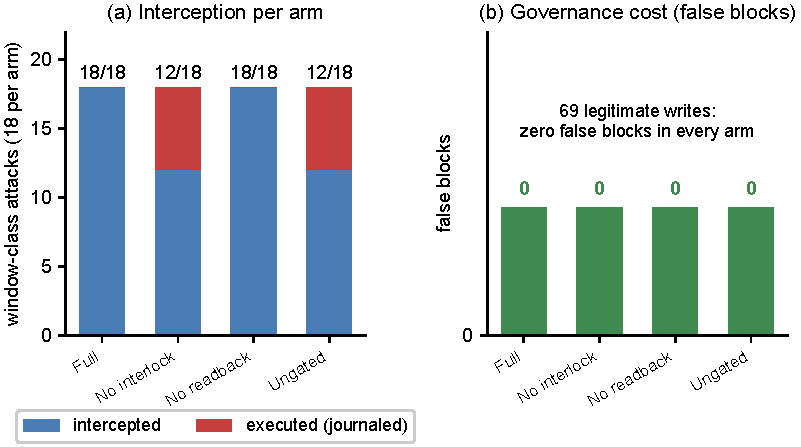
\includegraphics[width=0.98\columnwidth]{figures/fig3-ablation.pdf}
\caption{Mechanism attribution. (a)~Interception rate per repetition per
arm; only arms without the batch-window interlock admit the two
window-class attacks per repetition, and all executed breaches are
journaled. (b)~False blocks remain zero in every arm (the structural
hard range bounds writes without harassing legitimate traffic), and all
nine boundary probes pass in every arm.}
\label{fig:ablation}
\end{figure}

\subsection{Closed-loop case study on a running line (RQ3)}
\label{sec:eval-casestudy}

The flagship episode exercises the complete governed path on a running,
simulator-backed OPC UA production line (real protocol stacks, simulated
process physics): a melt-pumping unit of the cast-film scene
(physical-engine simulator with MES mirror). The goal is to bring the
three-minute mean melt pressure to at most 15.8\,MPa from an observed
16.1\,MPa, entirely through the platform's agent runtime: a lead agent
decomposing the goal and a governed write path with human approvals.
Acquisition on the target node ran at a median interval of 2.06\,s
(p90 2.09\,s, max 4.15\,s) with zero dropped windows over a one-hour
observation (1741 rows). The line had accumulated 22 batches, and the
model tier consumed a cross-run dataset of 15{,}989 rows over 7 runs.

Table~\ref{tab:casestudy} gives the decision timeline, reconstructed
from the audit ledger and approval records. The lead analyzed six
baseline windows (four shown: 16.04/16.00/15.99/16.01\,MPa) and
self-calibrated the process gain from observation (0.107--0.12\,MPa/rpm,
against 0.134 from historical data). It formed a proposal of
$130 \to 127$\,rpm, the largest single step the path would admit
(2\% of range), predicting 15.64--15.68\,MPa. Mid-flight, a second agent team restored a pending
proposal in the opposite direction. The one-proposal-in-flight gate
pinned it, and the lead located the conflict. A human arbitration
rejected the opposing proposal with a written basis rather than allowing
either team to force a write. The lead's proposal then entered the
governed path: the approval record bound the candidate value, the
applicable limits, and the active line--product--recipe--run tuple. A
human approved it. The write dispatched the same second and was
readback-verified at 127\,rpm. After process inertia, two retest windows
read 15.616 and 15.656\,MPa, within the goal and inside the
self-calibrated prediction band (measured gain 0.127\,MPa/rpm,
deviation 0.021--0.060 from the predicted band). A second approval
promoted the recipe version at 127\,rpm to prevent drift, and an
independent physical recheck read 15.5\,MPa with the setpoint read back
at 127\,rpm. The episode closed with the measured gain written back to
the channel's shared memory for future teams.

Two design behaviors surfaced on their own in this episode. First, the
model tier's dual-gate discipline held. A supervised surrogate model
trained on the line's own data passed all five promotion gates (single-
and rolling-horizon NRMSE 0.056 and 0.055 against bounds of 0.10 and
0.25; generalization gap 0.074 against 0.20; data volume and artifact
contract satisfied) and was promoted to shadow status. Yet the usage
gate refused it for model-driven MPC because its uncertainty-calibration
layer was absent, and the optimizer fell back to recommendation-only
operation with small safe steps. Model quality and permission to drive
control are deliberately different gates, and the episode shows the
distinction firing on a live model. Second, the episode exposed a real
product gap (the dataset builder could not replay control trajectories
from the write ledger into training data), which we report as a
limitation in Section~\ref{sec:discussion}.

A second, fully instrumented episode replicates the mechanical path with
an identified model: the omp RPC harness serving Qwen3.5-9B (64k context,
locally served) on a four-protocol cast-film scene against a production
build of the platform in an isolated instance. The agent's read task
returned values equal to device truth. A governed write then suspended
on a HITL card with the device value unchanged until the decision
(\emph{the interception is real, not nominal}); after approval, the
device register read exactly baseline$+3$ (195$\to$198), verified by
readback. A subsequent tuning task wrote a $+2.5$ adjustment
($198 \to 200.5$) with the melt-temperature PV converging toward the new
setpoint (intermediate sample 199.45\,°C; the closing review recorded a
settled deviation of 0.34\,°C). The parameter ledger attributed both
writes to the agent with their hypotheses. We note two boundaries
honestly: the human decision points in this replication were exercised
by an automated approver script (it validates the mechanical path, not
human judgment quality), and both episodes are single-scenario case
studies, not powered comparisons.

\begin{table}[!t]
\centering
\caption{Case-study decision timeline (melt-pressure correction on an
OPC UA line; all events ledger-reconstructed).}
\label{tab:casestudy}
\small
\begin{spacing}{1.0}
\begin{tabularx}{\columnwidth}{@{}p{0.16\columnwidth}X@{}}
\toprule
Time & Event \\
\midrule
00:36 & Goal dispatched (3-min mean melt pressure $\leq$15.8\,MPa; observed 16.1\,MPa) \\
00:54 & Cross-team arbitration: opposing in-flight proposal rejected by human with written basis \\
00:52--00:58 & Lead first round: six baseline windows (16.04/16.00/15.99/16.01\,MPa); self-calibrated gain 0.107--0.12\,MPa/rpm; proposal $130\to127$\,rpm (2\%-of-range step cap); predicted 15.64--15.68\,MPa \\
01:05:24 & Proposal enters governed path; approval record binds values, limits, and active tuple \\
01:05:27 & Human approval; dispatch same second; readback-verified at 127\,rpm \\
+inertia & Retest windows 15.616/15.656\,MPa $\leq$ 15.8; measured gain 0.127\,MPa/rpm inside prediction band \\
01:12:40 & Second approval promotes recipe version at 127\,rpm \\
post & Independent recheck: 15.5\,MPa; SP readback 127\,rpm; gain written back to channel memory \\
\bottomrule
\end{tabularx}
\end{spacing}
\end{table}

\subsection{Model-driven optimization tier (RQ4)}
\label{sec:eval-modeltier}

The optimization tier is evaluated in a live-loop configuration in which
an agent solves each beat against the governed solver and applies the
first move through the write path. Over a twelve-beat run with per-beat
context refresh, the median quality error fell from 6.42 to 0.02 (a
99.7\% reduction in this single twelve-beat run). Every manipulated
variable stayed inside its process window. In a twenty-seed paired
comparison, the tier solved 94.8\% of problem instances against 42.2\%
for static response-surface solving (rates aggregated over the paired
instances across seeds; per-seed denominators are in the frozen
artifact). This is a descriptive result consistent with the gated
model, not the solver alone, carrying the performance. Governance
semantics held
throughout. Solving without a qualified profile or binding is refused
with explanatory HTTP 409/422 status codes, and solver and twin must
agree on the same
frozen inputs to $10^{-6}$ relative tolerance. The full surface
survives a restart with bindings, profiles, and ledger intact
(seven persistence checks). Figure~\ref{fig:modeltier} summarizes these
results. These are simulation-tier results: the process models and the
twin are simulator-backed, and we do not claim plant-scale benefits.

\begin{figure}[!t]
\centering
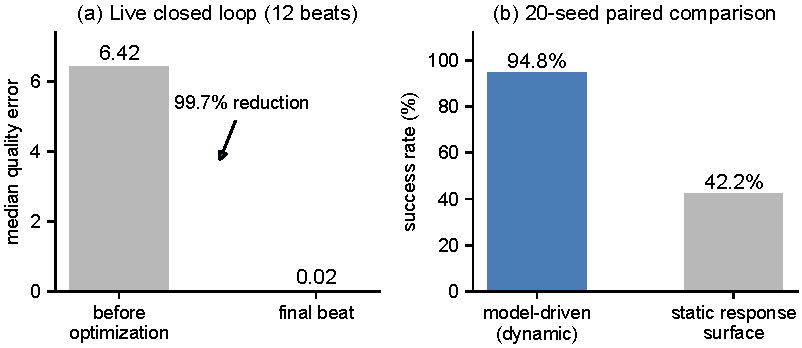
\includegraphics[width=0.98\columnwidth]{figures/fig4-modeltier.pdf}
\caption{Model-driven optimization tier. (a)~Median quality error over a
twelve-beat live closed loop: 6.42 before optimization to 0.02 at the
final beat (99.7\% reduction), with every MV inside its process window.
(b)~Twenty-seed paired comparison of dynamic model-driven solving versus
static response-surface solving: 94.8\% versus 42.2\% success.}
\label{fig:modeltier}
\end{figure}

\subsection{Adversarial containment (RQ5)}
\label{sec:eval-adversarial}

The final episode asks what happens when the model is genuinely weak and
the task genuinely hard. A three-agent team (lead plus two workers) on
the same 9B-class model, through the same harness, ran an injection-line
optimization goal under a production-like scenario. The episode's
qualification gates passed, but the workflow did not converge. The
platform behaved as designed throughout: the task was canceled
before completion, \emph{zero} unapproved writes reached the plant, and
the monitoring layer recorded twelve tool-surface violations and nine
unapproved harness tool calls. All were attributed and frozen with 153
raw event records and recomputed checksums. The process variable moved
31.28$\to$31.36\,g against a target of $32.5 \pm 0.35$\,g: the goal
was not achieved, and we report it as a negative result. The
governance-relevant observation is containment: a weak model was given a
supervisory task, misbehaved, and the platform's layered checks and
event monitors bounded the damage to zero plant writes while preserving
a complete evidentiary record. Two boundaries on this episode: no
prompt-injection attack was executed in it (the model misbehaved
unaided), so the telemetry-side injection threat of
Section~\ref{sec:problem-fm} remains to be exercised; and the episode is
a feasibility probe, not a powered comparison.

\subsection{Engineering quality and reproducibility (RQ1--RQ5)}
\label{sec:eval-quality}

Table~\ref{tab:quality} summarizes the regression base under the
behavioral results. The unit suite collects 915 tests with 913 passing
and two environment-skipped; line-governance, node-authority,
adversarial error handling, and security-check suites pass in full. A
frozen baseline captured from an earlier release is re-executed by the
benchmark runner: the four-arm ablation scenario reproduces bit-exactly
across a twelve-day gap (identical report hash). This is the property
that makes the ablation auditable after the fact. The same mechanism
honestly flags non-reproducibility elsewhere: a second baseline scenario
failed reproduction when the harness hash and source commit drifted, and
the runner reports that failure rather than masking it. Drift
detection is part of the evidence contract.

\begin{table}[!t]
\centering
\caption{Regression and evidence base underlying the behavioral results.}
\label{tab:quality}
\small
\begin{spacing}{1.0}
\begin{tabularx}{\columnwidth}{@{}p{0.42\columnwidth}X@{}}
\toprule
Suite & Result \\
\midrule
Unit tests & 913/915 pass (2 environment-skipped) \\
Line-governance end-to-end & 44/44 assertions \\
Node-authority surface & 52/52 \\
Adversarial error handling & 26/26 \\
Security hardening checks & 29/29 \\
Frozen-baseline reproduction (ablation scenario) & Bit-exact across 12 days \\
Frozen-baseline reproduction (second scenario) & Correctly reported NOT reproducible under commit/harness drift \\
\bottomrule
\end{tabularx}
\end{spacing}
\end{table}

\section{Discussion}
\label{sec:discussion}

\subsection{What the evidence establishes}
\label{sec:discussion-establishes}

The evaluation supports four claims at graded strength. Device-level
integration is established strongly (RQ1): five protocol stacks behave
identically on platform and device sides, including under faults, and the
behavior survives configuration changes and re-runs. Mechanism
attribution is established at the platform tier (RQ2). Its
epistemic status should be stated plainly: the ablation is an engineering
validation that the design's attribution story is true (the interlock
predicate does carry interception; the structural layers survive its
removal), not a causal comparison of governed against ungoverned
operation on plant outcomes. Such a comparison was deliberately not run
on a live path, and plant-KPI superiority is not claimed. What the
ablation does establish is defense in depth (the hard range survives
every disabled configuration) and the cost of governance on this
workload. The cost result is zero false blocks on injected legitimate
traffic. It is not a false-block rate for natural or adversarially
ambiguous plant traffic, and not a statement about in-range harmful
writes, such as compliant amplitudes applied at harmful times, which the
interval layers do not address. The closed-loop result (RQ3) is a feasibility demonstration
with unusually complete instrumentation: every decision is
ledger-reconstructed, approvals bind concrete tuples, and an independent
physical recheck corroborates the outcome. It is not a statistical
comparison, and one of its two episodes exercised the human decision
point with an automated approver. The adversarial result (RQ5) is a
negative-outcome containment case: it shows the platform bounding a weak
model's damage to zero writes, not that weak models can be made to
succeed. Throughout, the model-driven tier's benefits (RQ4) are
simulation-tier results by construction.

\subsection{Implications for practitioners}
\label{sec:discussion-practitioners}

Three lessons generalize beyond this implementation. First,
\emph{governance must live in configuration, not in prompts}. The same
agent surface that passed the ablation's legitimate traffic and blocked
its attacks never received a rule as text; the rules were intersections
of configuration facts. Teams deploying LLM agents against plants should
resist encoding limits in system prompts, which are advisory, and
instead make them admission predicates, which are enforceable.

Second, \emph{attribution is a first-class requirement, not a logging
by-product}. The ablation could identify the load-bearing layer only
because every layer records its own verdict. Operators debugging a
blocked write, or an auditor reconstructing an executed one, need
the excluding layer and the configuration revision, and they need
rejections recorded as faithfully as executions. The
\emph{attribution $\neq$ prevention} separation also has a practical
consequence: disabling a soft layer for commissioning does not blind the
audit, and a write that executes under a disabled interlock is still
visible.

Third, \emph{receipt grading changes what agents can honestly report}.
An agent that cites a readback-verified write and one that cites a
transport acknowledgment are making different claims; surfacing the
grade in the tool result makes the difference visible to the model and
to any human reading the report. This is the same discipline
human-factors research asks of automation: the human decision should be
exercised against concrete, inspectable evidence
\cite{parasuraman2000model}, not against a summary. The
complacency failure mode \cite{parasuramanmanzey2010complacency}
argues for keeping the approval payload specific enough that approving
is an informed act.

A deployment path follows from the architecture: commission bindings in
manual mode with batch-window interlocks on, review the ledger's
rejection records to tune limits, and promote individual bindings to
auto only after their rejection history is understood. The
configuration that the ablation exercised maps directly onto this
ramp-up.

For an application-oriented venue, the relevant question is whether the
governance layer survives deployment, not whether the underlying model is
stronger. The evaluation is deliberately staged: protocol-level fidelity
on real stacks, process-level behavior on a simulator, and plant-level
generalization as the next empirical step. The staging is a scope choice,
not a claim that simulation substitutes for a plant. A plant pilot should
start read-only, then move to single-point manual writes, then to bounded
automatic writes, keeping the same ledger and approval records throughout;
the protocol matrix and the four-layer path are the parts that transfer
unchanged.

\subsection{Limitations and threats to validity}
\label{sec:discussion-limits}

\textbf{Construct validity.} The ablation measures interception of
injected policy-breaching writes and false blocks on legitimate ones;
these are mechanistic constructs, not plant-outcome constructs. We do
not claim that governed supervision improves plant KPIs relative to
ungoverned supervision: that comparison was deliberately not run on a
live path, and the model-tier benefits are simulation-tier.

\textbf{External validity.} All plant contact is against simulator
backends: a physical-engine line simulator and a PLC node simulator
exposing real protocol stacks. The protocol behavior is real; the
process physics is simulated. The case-study line is single-site, and
the LLM episodes use one 9B-class open model family; stronger or
weaker models may shift where governance is exercised, though the
containment episode suggests the bound holds when the model is weak.

\textbf{Internal validity.} Case-study timelines are reconstructed from
the platform's own ledger; an independent log source does not exist for
these episodes (the physical recheck provides one external corroboration
point). The ablation's workload is synthetic by design, which is what
makes its attribution exact. Statistical-conclusion validity is
deliberately thin: most reported numbers are single-run or small-$n$
descriptive statistics, and we have marked each as such rather than
attaching tests they cannot support. Experimenter bias is a live
threat: the attack sets and legitimate workloads were designed by the
platform's authors with known expected outcomes, and no pre-registered
hypothesis test was run. The frozen-artifact discipline makes the
workloads auditable but not independent. Approval quality (whether human
approvers scrutinize records) is not measured; the replication episode's
scripted approver avoids claiming otherwise. Receipt grading under a
mis-applying device (a transport acknowledgment where the value is never
applied) is covered by design and by disconnect-fault checks, but no
experiment forced that exact failure; the readback-mismatch path
(re-reads, downgrade to unverified) is exercised by the
governance suite rather than by a dedicated plant-level probe.
Configuration governance is a further open side door: limits and recipe
windows are themselves configuration, and putting configuration changes
under the same approval-and-ledger discipline (management of change) is
future work. So is quantitative ramp-up guidance for the
manual-to-auto promotion path of
Section~\ref{sec:discussion-practitioners}.

\textbf{Reliability.} The frozen-baseline mechanism reproduced the
ablation bit-exactly across twelve days but correctly refused
reproduction on a drifted scenario, so regression claims are scoped to
commit- and hash-matched runs.

\textbf{Known product gaps.} The case study surfaced a real assembly
gap: the dataset builder derives control dimensions from acquisition
nodes only, so setpoint trajectories that live in the write ledger do
not yet flow into training data without an additional readback node.
The affected training path was locked closed by the twin gate rather
than producing an unsafe model. The audit ledger is append-only within
the platform process; externalizing it to write-once storage is future
work.

\section{Conclusion}
\label{sec:conclusion}

This paper treated the agent-to-plant write path (not the agent, and
not the chat) as the unit of governance for LLM-agent teams on
production lines. A configuration-driven binding model scopes agent
authority as a fact of plant structure; a four-layer admission interval
admits writes through independently inspectable boundaries; human
approval records bind exact proposals to tuples and are rechecked at
dispatch; receipt grading separates device-confirmed writes from
transport acknowledgments; and a total ledger records every decision,
including every rejection with its deciding layer.

The evaluation attributed interception to a specific layer with a
four-arm ablation (zero false blocks, executed breaches still journaled)
and demonstrated five-protocol device integration on real protocol stacks
with fault-honest behavior. It also showed a complete governed correction
on a running OPC UA line, from goal to self-calibrated proposal to human
approval to a readback-verified write that an independent recheck
corroborated. An adversarial episode showed a weak model's
out-of-surface behavior contained to zero plant writes. The
implementation is openly available, installs as a single service, and
reproduces its frozen ablation baseline bit-exactly under matched
commits.

Future work follows the limitations: replaying write-ledger trajectories
into training data so that the model tier can consume the platform's own
control history, externalizing the audit ledger to write-once storage,
and formal verification of the admission path's composition. Beyond
these, the agenda includes multi-site federations with shared governance
policy and replication of the closed-loop case study on physical plants
with measured approval workload for human experts.


\section*{Declaration of generative AI and AI-assisted technologies in the
writing process}
During the preparation of this work the authors used AI-assisted writing
tools in order to improve the language and structure of the manuscript.
After using these tools, the authors reviewed and edited the content as
needed and take full responsibility for the content of the published
article.

\section*{CRediT authorship contribution statement}
Author names are withheld for double-blind review. Individual contributions
follow the CRediT taxonomy (conceptualization, methodology, software,
validation, formal analysis, investigation, data curation, writing of the
original draft, review and editing, visualization, and supervision) and are
declared in full to the editorial system.

\section*{Declaration of competing interest}
The authors declare that they have no known competing financial interests or
personal relationships that could have appeared to influence the work
reported in this paper.

\section*{Data availability}
The platform implementation, configuration schemas, benchmark pipeline, and
the evidence artifacts for every experiment reported in Section~\ref{sec:eval}
are openly available. An anonymized repository link is provided to the
editorial system during double-blind review.

\bibliographystyle{elsarticle-harv}
\bibliography{resources/refs}

\end{document}
